\documentclass{article}
% generated by Madoko, version 1.0.0-rc5
%mdk-data-line={1}


\usepackage[heading-base={2},section-num={False},bib-label={True}]{madoko2}
\usepackage{xeCJK}
\usepackage{fontspec}
\usepackage{listings}


\begin{document}



%mdk-data-line={13}
\mdxtitleblockstart{}
%mdk-data-line={13}
\mdxtitle{\mdline{13}金融模型学习笔记}%mdk
\mdxauthorstart{}
%mdk-data-line={18}
\mdxauthorname{\mdline{18}吴子达}%mdk

%mdk-data-line={21}
\mdxauthoraddress{\mdline{21}格美熙资产管理}%mdk

%mdk-data-line={24}
\mdxauthoremail{\mdline{24}bleedtodry@hotmail.com}%mdk
\mdxauthorend\mdtitleauthorrunning{}{}\mdxtitleblockend%mdk
\mdline{15}
\begin{mdtoc}%mdk

\section*{Contents}\label{sec-contents}%mdk%mdk

\begin{mdtocblock}%mdk

\mdtocitemx{section}{\mdref{section}{1.\hspace*{0.5em}因子模型}}%mdk

\begin{mdtocblock}%mdk

\mdtocitemx{section}{\mdref{section}{1.1.\hspace*{0.5em}宏观经济因子模型}}%mdk

\mdtocitemx{section}{\mdref{section}{1.2.\hspace*{0.5em}基本面因子}}%mdk

\begin{mdtocblock}%mdk

\mdtocitemx{sec-fama-fench}{\mdref{sec-fama-fench}{1.2.1.\hspace*{0.5em}Fama-Fench三因子模型}}%mdk
%mdk
\end{mdtocblock}%mdk

\mdtocitemx{section}{\mdref{section}{1.3.\hspace*{0.5em}协方差矩阵}}%mdk

\mdtocitemx{section}{\mdref{section}{1.4.\hspace*{0.5em}主成分分析}}%mdk
%mdk
\end{mdtocblock}%mdk
%mdk
\end{mdtocblock}%mdk
%mdk
\end{mdtoc}%mdk

%mdk-data-line={17}
\section{\mdline{17}1.\hspace*{0.5em}\mdline{17}因子模型}\label{section}%mdk%mdk
\label{}%mdk
\noindent\mdline{18}\mdmathtag{(1)}\mdline{18}
\noindent\[%mdk-data-line={19}
\begin{aligned}
x &= \alpha+\beta f+\varepsilon  \\ 
E(\varepsilon) &= 0\\ 
E(f)&= 0\\ 
 cov(f,\varepsilon)&=0 \\ 
 cov(\varepsilon,\varepsilon)&= D,D=(\sigma_1^2,\cdots ,\sigma_1^N)I_N\\ 
 D&= diag(\sigma_1^2,\cdots ,\sigma_1^N)
\end{aligned}
\]%mdk
\noindent\mdline{28}假设条件:

%mdk-data-line={30}
\begin{itemize}[noitemsep,topsep=\mdcompacttopsep]%mdk

%mdk-data-line={30}
\item\mdline{30}残差项为均值为零的变量%mdk

%mdk-data-line={31}
\item\mdline{31}残差项彼此不相关%mdk

%mdk-data-line={32}
\item\mdline{32}残差项与因子之间彼此不相关%mdk

%mdk-data-line={33}
\item\mdline{33}残差项符合iid分布%mdk
%mdk
\end{itemize}%mdk

%mdk-data-line={35}
\subsection{\mdline{35}1.1.\hspace*{0.5em}\mdline{35}宏观经济因子模型}\label{section}%mdk%mdk

%mdk-data-line={36}
\noindent\mdline{36}宏观经济因子包括:%mdk

%mdk-data-line={38}
\begin{itemize}[noitemsep,topsep=\mdcompacttopsep]%mdk

%mdk-data-line={38}
\item\mdline{38}市场收益%mdk

%mdk-data-line={39}
\item\mdline{39}GDP增长率%mdk

%mdk-data-line={40}
\item\mdline{40}国债收益率%mdk

%mdk-data-line={41}
\item\mdline{41}通货膨胀率%mdk

%mdk-data-line={42}
\item\mdline{42}\dots{}\mdline{42}%mdk
%mdk
\end{itemize}%mdk

%mdk-data-line={44}
\noindent\mdline{44}例如我们对CPI residuals和IP residuals这两个宏观因子进行回归,得到下图:
\mdline{45}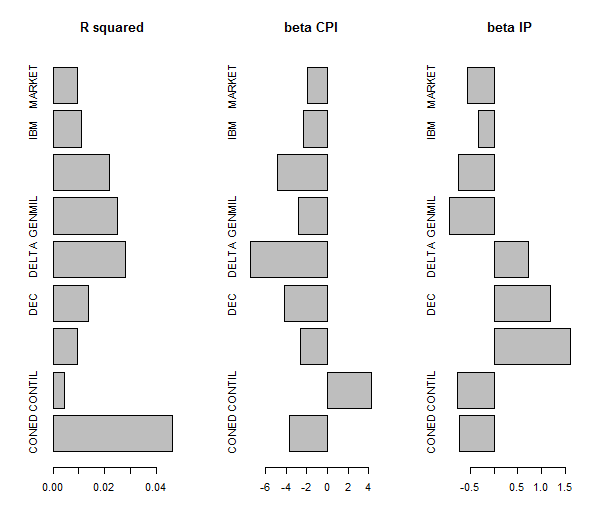
\includegraphics[keepaspectratio=true,width=\dimmin{}{\dimwidth{0.90}}]{images/Rplot}{}\mdline{45}%mdk

%mdk-data-line={49}
\noindent\mdline{49}上图中的R2指标非常小,说明股票对宏观因子的依耐性不显著,因此下一步分析我们转向
基本面因子。%mdk

%mdk-data-line={52}
\subsection{\mdline{52}1.2.\hspace*{0.5em}\mdline{52}基本面因子}\label{section}%mdk%mdk

%mdk-data-line={53}
\subsubsection{\mdline{53}1.2.1.\hspace*{0.5em}\mdline{53}Fama-Fench三因子模型}\label{sec-fama-fench}%mdk%mdk

%mdk-data-line={54}
\noindent\mdline{54}在因子模型中,最著名的莫过于1995年由Fama和Fench提出的三因子模型:%mdk
\label{}%mdk
\noindent\mdline{55}\mdmathtag{(2)}\mdline{55}
\noindent\[%mdk-data-line={56}
R_{j,t}-\mu_{f,t} = \beta_{0,j}+\beta_{1,j}(R_{M,t}-\mu_{f,t})+\beta_{2,j}SMB_t+\beta_{3,j}HML_t+\epsilon_t
\]%mdk

%mdk-data-line={59}
\begin{itemize}[noitemsep,topsep=\mdcompacttopsep]%mdk

%mdk-data-line={59}
\item\mdline{59}CAPM:市场组合的收益%mdk

%mdk-data-line={60}
\item\mdline{60}SMB: 一个投资组合中小盘股的收益减去大盘股的收益%mdk

%mdk-data-line={61}
\item\mdline{61}HML:一个投资组合中高账面市值比股票的收益减去低账面市值比股票的收益%mdk
%mdk
\end{itemize}%mdk

%mdk-data-line={65}
\subsection{\mdline{65}1.3.\hspace*{0.5em}\mdline{65}协方差矩阵}\label{section}%mdk%mdk

%mdk-data-line={66}
\noindent\mdline{66}由于\mdline{66}$x-\alpha=\beta f+\varepsilon$\mdline{66},所以收益的协方差矩阵为:%mdk
\label{}%mdk
\noindent\mdline{67}\mdmathtag{(3)}\mdline{67}
\noindent\[%mdk-data-line={68}
\sum=E[(x-\alpha)(x-\alpha)^`]
\]%mdk
\noindent\mdline{70}因子模型中使用的都是风险模型。每一时刻\mdline{70}$t$\mdline{70}的收益被解释为\mdline{70}$t$\mdline{70}时刻的给定因子的线性组合。
暴露于共同因子的由收益方差所度量的风险为不可分散风险——无论我们所选择的投资组合有多大,
该风险都无法被分散。如果解释\mdline{72}$t$\mdline{72}时刻的因子在\mdline{72}$t-1$\mdline{72}时刻是可以被预测的,那么因子模型就
可以用来预测收益。因子模型一般分为三类:统计因子,基本面因子和宏观因子。

%mdk-data-line={74}
\subsection{\mdline{74}1.4.\hspace*{0.5em}\mdline{74}主成分分析}\label{section}%mdk%mdk

%mdk-data-line={80}
\begin{mdbmargintb}{4em}{}%mdk
\begin{mdflushright}%mdk
{\tiny\mdline{81}Created with~\href{https://www.madoko.net}{Madoko.net}.}%mdk
\end{mdflushright}%mdk
\end{mdbmargintb}%mdk%mdk


\end{document}
